\documentclass[tikz,convert={outfile=\jobname.svg}]{standalone}
\usetikzlibrary{calc,patterns,snakes}
% \usetikzlibrary{...}% tikz package already loaded by 'tikz' option
\begin{document}
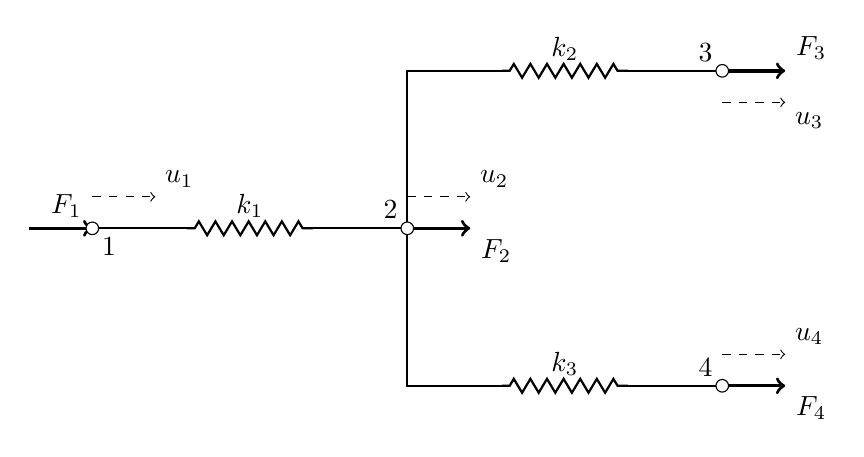
\begin{tikzpicture}[scale=0.4]
    \tikzstyle{spring}=[thick,decorate,decoration={zigzag,pre
        length=0.1cm,post length=0.1cm,segment length=6}]
    % Springs-Lines
    \draw[thick] (0,0) -- (3,0);
    \draw[spring] (3,0) -- (7,0) node[above,pos=0.5] {$k_1$};
    \draw[thick] (7,0) -- (10,0); \draw[thick] (10,0) -- (10,5) -- (13,5);
    \draw[thick] (10,0) -- (10,-5) -- (13,-5);
    \draw[spring] (13,5) -- (17,5) node[above,pos=0.5] {$k_2$};
    \draw[spring] (13,-5) -- (17,-5) node[above,pos=0.5] {$k_3$};
    \draw[thick] (17,5) -- (20,5); \draw[thick] (17,-5) -- (20,-5);
    % Forces and DOFs
    \draw[very thick,->] (-2,0) -- (0,0) node[above left] {$F_1$};
    \draw[very thick,->] (10,0) -- (12,0) node[below right] {$F_2$};
    \draw[very thick,->] (20,5) -- (22,5) node[above right] {$F_3$};
    \draw[very thick,->] (20,-5) -- (22,-5) node[below right] {$F_4$};
    \draw[dashed,->] (0,1) -- (2,1) node[above right] {$u_1$};
    \draw[dashed,->] (20,4) -- (22,4) node[below right] {$u_3$};
    \draw[dashed,->] (10,1) -- (12,1) node[above right] {$u_2$};
    \draw[dashed,->] (20,-4) -- (22,-4) node[above right] {$u_4$};
    % Nodes
    \draw[fill = white] (0, 0) circle (.2) node[below right] {$1$};
    \draw[fill = white] (20,5) circle (.2) node[above left] {$3$};
    \draw[fill = white] (10,0) circle (.2) node[above left] {$2$};
    \draw[fill = white] (20,-5) circle (.2) node[above left] {$4$};
  \end{tikzpicture}
\end{document}